\documentclass[14pt]{extarticle}
\input{external/preamble-latex-cools.tex}
\begin{document}
\begin{project}{Actividad de cierre}{Encuentra el producto desconocido.}{cool-encuentraProductoDesconocido}%
¿Qué número debería ir en lugar del signo de interrogación? Explica o muestra tu razonamiento.%
\begin{image}{0}{1}{0}{}%
\includegraphics[max width=\linewidth, center]{external/svg-source/tikz-file-153040-scale13.pdf}
\end{image}%
\begin{image}{0}{1}{0}{}%
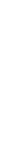
\includegraphics[max width=\linewidth, center]{external/whitespace-tikz/3cm.pdf}
\end{image}%
\end{project}
\end{document}